\section{Implementation \& Design}
\label{sec:implem}
  For this paper the Fibonacci and the Sort algorithm from BOTS are chosen to be implemented, as introduced in subsection \ref{subsec:BOTS}.
  Additionally, a generic algorithm is implemented.
  All three are implemented using OpenMP, HPX and in a sequential way.
  
  \paragraph{Fibonacci}
  The algorithm can spawn a high amount of tasks with small workload.
  The workload of forking and joining new threads and scheduling this amount of tasks might have the biggest impact when it comes to performance.
  
  The implementation is done without cut offs for the HPX and OpenMP versions.
  This means that every recursive call of the Fibonacci function creates a new task.
  \begin{lstlisting}[
  caption=Fibonacci OpenMP Implementation,
  label=lst1:fibOMP,
]
long long fibonacci(long long input) {
    if (input < 2 ) return input;
    long long x, y;
    #pragma omp task shared(x) firstprivate(input)
    x = fibonacci(input - 1);
    #pragma omp task shared(y) firstprivate(input)
    y = fibonacci(input - 2);
    #pragma omp taskwait
    return x + y;
}
\end{lstlisting}
  Listing \ref{lst1:fibOMP} shows a first implementation of the Fibonacci algorithm using OpenMP.
  It shows which directives are used.
  As explained in subsection \ref{subsec:OpenMP}, the \texttt{\#pragma omp task} directive creates a new task which may be executed.
  Using the \texttt{shared} and \texttt{firstprivate} clauses adjusts the variable scopes so that each task has its own instance of the parameter input.
  Variables \texttt{x} and \texttt{y} are shared which means no new instance is created.
  At the end the \texttt{\#pragma omp taskwait} directive tells the function to wait until all the child tasks finished their execution.
  
\begin{lstlisting}[
  caption=Fibonacci HPX Implementation,
  label=lst1:fibHPX,
]
long long fibonacci(long long input) {
  if (input < 2) return input;
  hpx::future<long long> n1 =
      hpx::async(fibonacci, input - 1);
  hpx::future<long long> n2 = 
      hpx::async(fibonacci, input - 2);
  return n1.get() + n2.get();
}
\end{lstlisting}
  The HPX implementation of the Fibonacci algorithm can be seen in listing \ref{lst1:fibHPX}.
  In contrast to OpenMP, HPX works with futures to abstract results of function calls.
  Calling a function with \texttt{hpx::async} creates a task and immediately returns a future to continue the execution.
  Calling \texttt{get} on a future suspends the current thread until this future is returned.
  \\
 
  \paragraph{Merge Sort}
  The Sort algorithm of BOTS is slightly adjusted to a normal Merge Sort.
  It is a suitable use case, easy to implement and can also spawn a high number of tasks.
  Similar to Fibonacci Merge Sort is also implemented without cut off. 
  \\
  
  \paragraph{Generic Algorithm}
  The aim of this algorithm is to enable task size adjustment and allow to define the number of tasks easily by parameters.
  
  The algorithm uses two arrays which sizes are defined at the building process.
  First of all one array is filled by randomized floating point numbers.
  To compare each run a deterministic seed for the random numbers is chosen.
  In each turn the element of a vector is equal to a calculation on the element of the other array as it can be seen in a) of figure \ref{fig:gen_algo}.
  The sinus function is calculated on the element before it is multiplied by ten and adjusted to an absolute value.
  This turns are repeated a defined number of times.
  
  The task size can be adapted by parameters and defines how many array elements are calculated by a task.
  The task size furthermore defines how many tasks are used per run.
  This number is equal to the array size divided by the task size.
  As each turn depends on the execution of the previous turn, synchronization is done only at the end of a turn.
    
\begin{figure}[htbp]
	\centering
	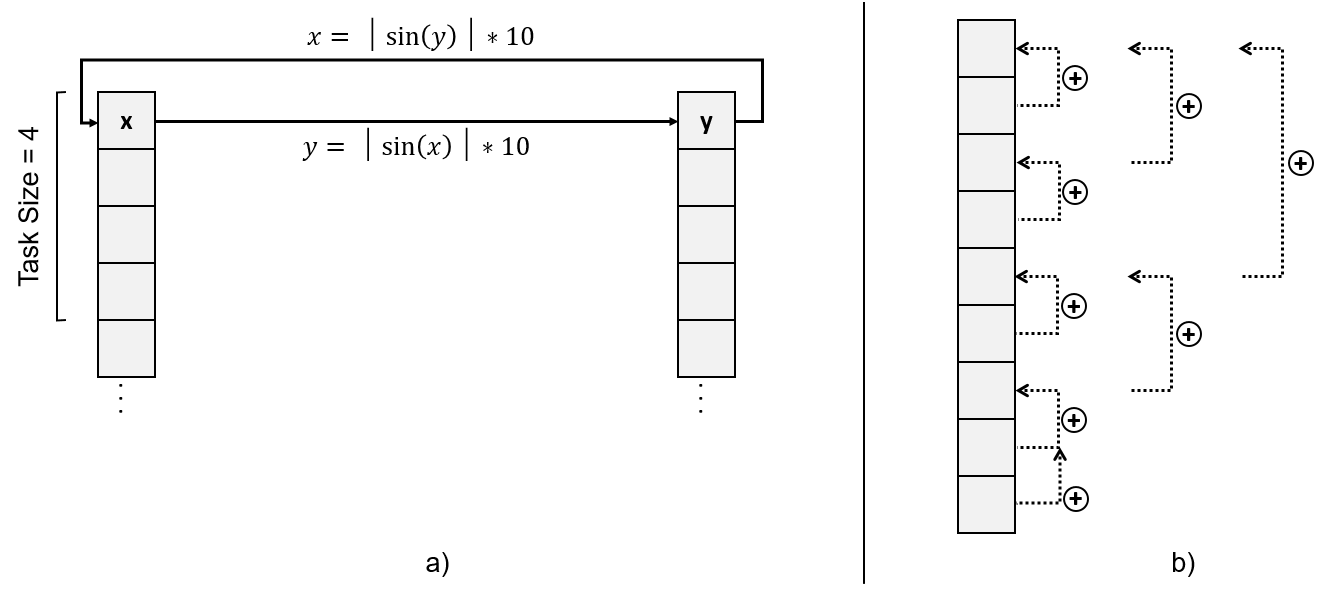
\includegraphics[width=0.48\textwidth]{figures/generic_alorithm.PNG}
	\caption{Generic Algorithm a) Turns b) Summation}
	\label{fig:gen_algo}
\end{figure}

  After the last turn is executed, all elements of the last calculated array are summed up.
  This is done by building pairs and adding the value of the second member to the value of the first one and storing the results in the first value's element.
  Part b of figure \ref{fig:gen_algo} illustrates how these pairs are arranged.
  It also shows how elements are handled that cannot be part of a pair.
  These leftover element is added to the result of the last pair.
  This process is continued with the resulting values until only one element is left.
\\

The code can be found on GitHub~\cite{t0BEE.2020}.
It is mainly written in C++, but also contains CMake files and scripts for building, execution, and formatting the results.
